%Τα μαθηματικά εργαλία που παρουσιάζονται σε αυτό το κεφάλαιο %εμπίπτουν στον τανυστικό λογισμό. 
Στο πλαίσιο της γενικής θεωρίας της σχετικότητας, ένα βαρυτικό πεδίο αντικαθίσταται με ένα καμπυλομένο χωρόχρονο, ή μια διαφορίσιμη πολλαπλότητα. Η καμπυλότητα του χωροχρόνου που συνδέεται με τις βαρυτικές δυνάμεις περιγράφεται από τον τανυστή καμπυλότητας του Riemann.
\\ 
%Η άμεση ταύτιση της καμπυλότητας με καμπύλες επιφάνειες %εμβαπτισμένες στον τρισδιάστατο ευκλείδειο χώρο απομακρύνει από %τη δέουσα ερμηνεία και επισκιάζει το ευρύτερο σύνολο καμπύλων %χώρων.

\section{Μετασχηματισμοί συντεταγμένων}
%Η γενικά μη ευκλείδεια γεωμετρία του χωροχρόνου λοιπόν, σε %συνδυασμό με την ανάγκη για αυθαιρεσία ως προς το σύστημα %συντεταγμένων
Οι εξισώσεις φυσικών νόμων και φυσικά μεγέθη όπως το μήκος και ο ιδιοχρόνος πρέπει να παραμένουν αναλλοίωτα ως προς γενικούς μετασχηματισμούς συντεταγμένων. Με βάση τον κανόνα της αλυσίδας, οι απειροστές μεταβολές των νέων και των αρχικών συντεταγμένων ικανοποιούν τη σχέση 
%Καθοριστική ιδιότητα αυτών των αντικειμένων είναι ο %μετασχηματισμός τους κάτω από αλλαγή του συστήματος %συντεταγμένων 
\begin{equation}\label{dtransf}
    d\y\indices{^\mu} \,=\, \frac{\partial \y\indices{^\mu}}{\partial x\indices{^\nu}}\,dx\indices{^\nu}
\end{equation}
όπου οι ελληνικοί δείκτες αναφέρονται στις διαστάσεις του χωροχρόνου, με το δείκτη $0$ να αντιστοιχεί στην χρονική διάσταση.
Τα διανυσματικά μεγέθη 
%\footnote{Παρουσιάζονται μετασχηματισμοί ενός τανυστή Τ, πρώτης %τάξεως, από το σύστημα συντεταγμένων $x\indices{^\mu}$ στο %σύστημα $\y\indices{^\mu}$. Στο σύστημα $\y\indices{^\mu}$ ο Τ %τονίζεται για σαφήνεια.} 
κατατάσσονται σε δύο είδη: τα ανταλλοίωτα διανυσματικά μεγέθη
\begin{equation}
    T'^{\mu}\,=\,\frac{d\y^{\mu}}{dx^{\nu}}\,T^{\nu}
\end{equation}
και τα συναλλοίωτα
\begin{equation}
    T'_{\mu}\,=\,\frac{dx^{\nu}}{d\y^{\mu}}\,T_{\nu}
\end{equation}
Οι πιο πάνω μετασχηματισμοί γενικεύονται και στην περίπτωση τανυστών ανώτερης τάξης, όπου εμφανίζεται ένας ανταλλοίωτος πίνακας μετασχηματισμού για κάθε πάνω δείκτη και ένας συναλλοίωτος για κάθε κάτω δείκτη.
\\

Επειδή οι πιο πάνω μετασχηματισμοί είναι γραμμικοί, εάν ένας τανυστής μηδενίζεται σε ένα σύστημα αναφοράς, θα μηδενίζεται σε κάθε σύστημα αναφοράς. Ισχύει επίσης και το αντίστροφο - μια ποσότητα (με πολλές συνιστώσες) που μηδενίζεται σε κάποιο σύστημα αλλά όχι σε κάποιο άλλο δεν είναι τανυστής. 

\section{Πολλαπλότητα Riemann}
Προς το παρόν, περιγράφουμε $N$-διάστατες χωρικές πολλαπλότητες Riemann. Το αναλλοίωτο απειροστό διάστημα μεταξύ γειτονικών σημείων ισούται με
\begin{equation}\label{dlength}
    ds^2 = \g{\mu}{\nu}dx\indices{^\mu}dx\indices{^\nu} 
\end{equation}
όπου $\g{\mu}{\nu}$ η μετρική. Το απειροστό αυτό διάστημα πρέπει να είναι θετικό, επομένως όλες οι ιδιοτιμές της μετρικής είναι θετικές.
%Εδώ, οι ελληνικοί δείχτες παίρνουν τιμές 1-N αφού δεν υπάρχει χρονική συνιστώσα και χρησιμοποιούνται παράλληλα με τους αγγλικούς. 
Στην περίπτωση ενός χωροχρόνου, το απειροστό διάστημα \eqref{dlength} μπορεί να είναι θετικό, αρνητικό ή ακόμη και μηδενικό. Οπότε μια ιδιοτιμή της μετρικής είναι αρνητική. \\

Με βάση την αναλλοιότητα του απειροστού διαστήματος μπορούμε να εξαγάγουμε το μετασχηματισμό της μετρικής $\g{\mu}{\nu}$, χρησιμοποιώντας την \eqref{dtransf} και την \eqref{dlength}
\begin{equation}
\begin{split}
    ds^2 &= \g{\mu}{\nu} dx\indices{^\mu}dx\indices{^\nu}\\
        &= \underbrace{\g{\mu}{\nu} \L[1]{\mu}{\alpha} \L[1]{\nu}{\beta}}_{\g{\alpha}{\beta}'} d\y\indices{^\alpha}d\y\indices{^\beta}
\end{split}
\end{equation}
Άρα λοιπόν η μετρική στο νέο σύστημα αναφοράς συντεταγμένων $\y\superscr{\mu}$ ικανοποιεί 
\begin{equation}\label{metrictrans}
    \g{\alpha}{\beta}'(\y)  \,=\, \g{\mu}{\nu}(x) \L[1]{\mu}{\alpha} \L[1]{\nu}{\beta}
\end{equation}

\section{Βαθμοί ελευθερίας της μετρικής}
Γενικά, τα $N^2$ στοιχεία της μετρικής $\g{\alpha}{\beta}$ αποτελούν συνεχείς, διαφορίσιμες συναρτήσεις των συντεταγμένων σε κάθε σημείο του χωροχρόνου. Επειδή η μετρική είναι ένας συμμετρικός τανυστής, ο αριθμός των ανεξάρτητων στοιχείων της είναι μικρότερος. Με βάση τον ορισμό του απειροστού διαστήματος \eqref{dlength}, το αντισυμμετρικό μέρος μπορεί να αμεληθεί. %Δεδομένου ότι, μια γενική μετρική μπορεί πάντα να γραφτεί ως το %άθροισμα ενός συμμετρικού και ενός αντισυμμετρικού όρου
%\begin{equation*}
%    \g{\alpha}{\beta} \,=\,  %\underbrace{\frac{\g{\alpha}{\beta}+\g{\beta}{\alpha}}{2}}_{S\i%ndices{_\alpha_\beta}}+\underbrace{\frac{\g{\alpha}{\beta}-\g{\%beta}{\alpha}}{2}}_{A\indices{_\alpha_\beta}}
%\end{equation*}
%αντικαθιστώντας το πιο πάνω στην \eqref{dlength}, βλέπουμε ότι %δεν υπάρχει συνεισφορά από το $A\indices{_\alpha_\beta}$ 
%\begin{equation*}
%    A\indices{_\alpha_\beta}dx\indices{^\alpha}dx\indices{^\beta} \,=\, - A\indices{_\beta_\alpha}dx\indices{^\alpha}dx\indices%{^\beta} \,=\,  -A\indices{_\alpha_\beta}dx\indices{^\alpha}dx\%indices{^\beta} \,=\,0
%\end{equation*}
Άρα λοιπόν θεωρούμε μόνο συμμετρικές μετρικές με πλήθος στοιχείων
\begin{equation}\label{smetricdof}
    \frac{N}{2}\left( N+1 \right)
\end{equation}

\section{Τοπικά επίπεδο σύστημα συντεταγμένων}\label{sec_localcartcoor}
%Έχοντας λοιπόν στη διάθεση μας, τους μετασχηματισμούς ως προς %συστήματα συντεταγμένων για Riemannian πολλαπλότητες %\eqref{metrictrans}, είμαστε σε θέση 
Θα αποδείξουμε τώρα ότι δεν υπάρχει μετασχηματισμός αλλαγής συντεταγμένων, $x\indices{^\mu}\rightarrow \y\indices{^\nu}$, που να μετασχηματίζει μια μετρική σε μια γενική, καμπυλομένη πολλαπλότητα στην επίπεδη ευκλείδεια μετρική, δηλαδή
\begin{equation}\label{gtodelta}
     \g{\mu}{\nu}'(\y) \,=\, \g{\mu}{\nu}(x) \L[1]{\mu}{\alpha} \L[1]{\mu}{\beta} \,\rightarrow\, \de\indices{_\mu_\nu}  
\end{equation}
σε κάθε σημείο της πολλαπλότητας \cite{Carroll2003-CARSAG-3}. 
%το διαφορικό μήκος ευκλείδειας μορφής
%\begin{equation*}
%     ds^2 = \de\indices{_\mu_\nu} %d\y\indices{^\mu}d\y\indices{^\nu}
%\end{equation*}
Οι $\frac{N}{2}(N+1)$ συνθήκες της \eqref{gtodelta} δεν μπορούν να ικανοποιηθούν με βάση τους $Ν$ μετασχηματισμούς αλλαγής συντεταγμένων: $x\indices{^\mu}(\y^\nu)$. Παρόλα αυτά, είναι δυνατόν να ικανοποιήσουμε ένα άλλο σύνολο συνθηκών, με βάση τις οποίες η μετρική ανάγεται στην ευκλείδεια μετρική σε μια αρκετά μικρή περιοχή γύρω από ένα αυθαίρετο σημείο $P$ της πολλαπλότητας:
\begin{equation}
    \lim_{\y\rightarrow \y_P} ds\superscr{2} \,=\,  \de\indices{_\mu_\nu} d\y\indices{^\mu}d\y\indices{^\nu}
\end{equation}
Η ιδιότητα αυτή των πολλαπλοτήτων Riemann είναι άμεσα συνιφασμένη με την αρχή της ισοδυναμίας του Einstein. Αναφερόμαστε στο ζητούμενο σύστημα $y$ ως το τοπικά αδρανειακό σύστημα αναφοράς.\\

%Αν και το σύστημα $\y\indices{^\mu}$ είναι αρχικά άγνωστο, 
Αναπτύσσουμε τις συναρτήσεις μετασχηματισμού κατά Taylor γύρω από το σημείο P, το οποίο, στο αρχικό σύστημα αναφοράς περιγράφεται από τις συντεταγμένες $x\superscr{\mu}\subscr{P}$:
\begin{equation}
    x\indices{^\mu}(\y) \,=\, x\superscr{\mu}\subscr{P} \,+\, \left( \frac{\partial x\superscr{\mu}}{\partial \y\superscr{a}} \right)_P\,\y\superscr{a} \,+\, \frac{1}{2}\left( \frac{\partial\superscr{2} x\superscr{\mu}}{\partial \y\superscr{a} \partial \y\superscr{b}} \right)_{P} \y\superscr{a} \y\superscr{b} \,+\, \dots
\end{equation}
Σε κάθε όρο στο πιο πάνω αναπτύγμα εμφανίζονται ελεύθερες παραμέτροι, των οποίων ο αριθμός καθορίζεται με βάση τη μεταθετικότητα των μερικών παραγώγων. Παραδείγματος χάριν, οι πρώτες μερικές παράγωγοι 
\begin{equation}\label{secterm}
    \frac{\partial x\superscr{\mu}}{\partial \y\superscr{a}}
\end{equation}
αντιστοιχούν σε πίνακα με $N^2$ ανεξάρτητα στοιχεία, τα οποία, προσδιορίζουν τις απαραίτητες συναρτήσεις μετασχηματισμού σε μια αρκετά μικρή περιοχή γύρω από το σημείο $P$. Σε μεγαλύτερες περιοχές, συνεισφέρουν όροι μερικές παράγωγοι ανώτερης τάξης, όπως 
\begin{equation}\label{thrterm}
    \frac{\partial\superscr{2} x\superscr{\mu}}{\partial \y\superscr{a} \partial \y\superscr{b}}
\end{equation}
Εξαιτίας της αναλλοιώτητας ως προς την εναλλαγή των δύο κάτω δεικτών, οι δεύτερες μερικές παράγωγοι ανάγονται σε $\frac{N^2}{2}(N+1)$ επιπρόσθετους βαθμούς ελευθερίας. Καθορίζοντας τις παραγώγους στο $P$, βρίσκουμε τις αναγκαίες συναρτήσεις μετασχηματισμού για να ικανοποιήσουμε τις ζητούμενες συνθήκες που πρέπει να πληροί η μετρική στο νέο σύστημα αναφοράς συντεταγμένων.\\

Με τον ίδιο τρόπο αναπτύσσοντας τη μετρική ως προς $y$. 
%θα καταλ΄ληξουμε σε σημαντικά συμπεράσματα. 
Για απλοποίηση των εκφράσεων, επιλέγουμε το σημείο $P$ να συμπίπτει με το σημείο αναφοράς και των δύο συστημάτων, $x\superscr{\mu}\subscr{P} = \y\superscr{\mu}\subscr{P}=0$.  Αναπτύσσουμε τα δύο μέλη της \eqref{metrictrans} 
%με σκοπό την σύγκριση, αριστερά και δεξιά της ισότητας, των %όρων ίδιας τάξης 
ως προς y και παίρνουμε
\begin{equation}\label{tayloroftrans}
    \begin{split}
        \g{\mu}{\nu}'(P) &\,+\, \left( \pd{\g{\mu}{\nu}'}{\y\superscr{a}} \right)_P  \y\superscr{a} \,+\, \frac{1}{2}\left( \spd{\g{\mu}{\nu}'}{\y\superscr{a}}{\y\superscr{b}} \right)_P \y\superscr{a}\y\superscr{b} \,+\,\dots \\ \\
        &=\, \left( \pd{x\superscr{\rho}}{\y\superscr{\mu}}\pd{x\superscr{\sigma}}{\y\superscr{\nu}}\g{\rho}{\sigma} \right)_P \,+\, \left( \pd{x}{\y}\spd{x}{\y}{\y}g \,+\, \dots \right)_P  \y\superscr{a} \,+\, \frac{1}{2}\left( \frac{\partial x}{\partial\y}\frac{\partial\superscr{3}x}{\partial\y\partial\y\partial\y}g + \dots \right)_P \y\superscr{a}\y\superscr{b}\,+\,\dots
    \end{split}
\end{equation}

Για λόγους απλότητας, δεν παραθέτουμε τους δείκτες στο δεξιό μέλος της \eqref{tayloroftrans}. 
%όπως επίσης και όροι παραγώγων επαναλαμβανόμενης τάξεως. 
%\newpage
Συγκρίνοντας τους όρους μηδενικής τάξεως ως προς $y$, 
%δεξιά και αριστερά, 
συμπερένουμε ότι μπορούμε στο σημείο $P$ να μετασχηματίσουμε τη μετρική στη μορφή που θέλουμε. Ο ζητούμενος μετασχηματισμός ροσδιορίζει ένα τοπικά επίπεδο σύστημα συντεταγμένων, δηλαδή
\begin{equation}\label{firstcond}
     \g{\mu}{\nu}'(P) = \de\indices{_\mu_\nu} \qquad \de\indices{_\mu_\nu} := \rm{diag}(+1,+1,\dots)
\end{equation}
και στην περίπτωση του χωροχρόνου ένα τοπικά αδρανειακό σύστημα αναφοράς συντεταγμένων
\begin{equation*}
     \g{\mu}{\nu}'(P) = \mink{\mu}{\nu} \qquad \mink{\mu}{\nu} := \rm{diag}(-1,+1,\dots)
\end{equation*}
Οι συνθήκες (εξισώσεις) που πρέπει να ικανοποιηθούν για το καθορισμό του μετρικού πίνακα $\g{\mu}{\nu}'$ στο σημείο P είναι $\frac{N}{2}(N+1)$ ακριβώς όσοι και οι βαθμοί ελευθερίας \eqref{smetricdof}. Ο όρος στα δεξιό μέλος
\begin{equation*}
    \pd{x\superscr{\rho}}{\y\superscr{\mu}}\pd{x\superscr{\sigma}}{\y\superscr{\nu}}\g{\rho}{\sigma}
\end{equation*}
μας προμηθεύει με $N^2$ ελεύθερες παραμέτρους, με τις οποίες μπορούμε να ικανοποιήσουμε τις εξισώσεις \eqref{firstcond}. Περισσεύουν
\begin{equation}\label{SONdof}
    \frac{N}{2}(N-1)
\end{equation}
παραμέτροι οι οποίες αντιστοιχούν στις παραμέτρους των περιστροφών της ομάδας SO(N) που αφήνουν αναλλοίωτη την ευκλείδεια μετρική $\de\indices{_\mu_\nu}$. 
%- συγκεκριμένα ισχύει
%\begin{equation*}
%    R\indices{^\alpha_\rho}R\indices{^\beta_\sigma}\de\indices{%^\rho^\sigma} \,=\, \de\indices{^\alpha^\beta}
%\end{equation*}
%Η επέκταση των προαναφερόμενων, εντός πολλαπλότητας %pseudo-Riemann με a χρονικές και b χωρικές διαστάσεις, είναι %άμεση. Με την αναλυτική συνέχεια των 'a'  διαστάσεων από τις N
%\begin{equation*}
%    x\subscr{1}\rightarrow i x\subscr{1},\quad %x\subscr{2}\rightarrow i x\subscr{2}, \quad\dots
%\end{equation*}
%η ομάδα SO(N) αντικαθίσταται από την SO(a,b), της οποίας η %άλγεβρα κατασκευάζεται επίσης από $\frac{N}{2}(N-1)$ %γεννήτορες. Τα στοιχεία της ομάδας δρουν στο διαφορικό %$dx\indices{^\mu}$
%\begin{equation*}
%    d\y\indices{^\mu} \,=\, L\indices{^\mu_\nu} %dx\indices{^\nu}
%\end{equation*}
%εντούτοις, αφήνουν αναλλοίωτο το τετράγωνο της απόστασης
%\begin{equation*}
%    ds^2 \,=\, -\sum\limits_{i=1}^{\text{a}}(dx\indices{^i})^2 %\,+\, \sum\limits_{i=\text{a}+1}^{\text{a+b}}(dx\indices{^i})^2
%\end{equation*}
%ή ισοδύναμα
%\begin{equation*}
%    L\indices{^\alpha_\rho}L\indices{^\beta_\sigma}\mink{\rho}{%\sigma} \,=\, \mink{\alpha}{\beta}
%\end{equation*}
%Ακόμη όμως, δεν αποδείχθηκαν οι δύο ισχυρισμοί που έγιναν στην %αρχή της ενότητας. 
\\

Συνεχίζοντας με τον ίδιο τρόπο, 
%αρίθμησης των βαθμών ελευθερίας, 
συγκρίνουμε τους όρους πρώτης τάξης ως προς $y$, στο αριστερό και δεξιό μέλος της \eqref{tayloroftrans}. %\newpage
Αυτό μας επιτρέπει να εξετάσουμε μια πολύ μικρή περιοχή γύρω από το σημείο $P$, έτσι ώστε ο όροι ανώτερης τάξης των αναπρυγμάτων να είναι αμελητέοι. Για να επιτύχουμε την κατασκευή ενός τοπικά επίπεδου ή τοπικά αδρανειακού συστήματος στην περιοχή αυτή, επιβάλλουμε
\begin{equation}\label{seccond}
     \pd{\g{\mu}{\nu}'}{\y\superscr{a}} = 0
\end{equation}
το οποίο αντιστοιχεί με 
\begin{equation}
     \frac{N^2}{2}(N+1)
\end{equation}
συνθήκες. 
%οι οποίες πρέπει να ικανοποιηθούν ρυθμίζοντας ανάλογα τις %συναρτήσεις μετασχηματισμών. 
Στο δεξιό μέλος της \eqref{tayloroftrans} ο όρος πρώτης τάξης περιέχει $\frac{N^2}{2}(N+1)$ ελεύθερες παραμέτρους, αρκετές  για να ικανοποιήσουμε τις συνθήκες \eqref{seccond}.
\\

%Μέχρι τώρα, έγινε επιβολή των συνθηκών \eqref{firstcond} και %\eqref{seccond} χωρίς κανένα πρόβλημα απροσδιοριστίας. Έχουμε %τόσες συνθήκες όσες και ανεξάρτητες  παραμέτρους. 

Το επόμενο σύνολο συνθηκών που πρέπει να ικανοποιήσουμε προέρχεται από τον όρο δεύτερης τάξης ως προς $y$, στο αριστερό μέλος της \eqref{tayloroftrans} 
\begin{equation}
    \spd{\g{\mu}{\nu}'}{\y\superscr{a}}{\y\superscr{b}} \,=\, 0
\end{equation}
και δίνει 
\begin{equation*}
    \frac{N^2}{4}(N+1)^2
\end{equation*}
ανεξάρτητες εξισώσεις. Στο δεξιό μέλος υπάρχουν επίσης όροι δεύτερης τάξης ως προς $y$. Στους όρους αυτούς οι πρώτες και δεύτερες μερικές παράγωγοι έχουν ήδη καθοριστεί. Οι τρίτες μερικές παράγωγοι  
\begin{equation}
    \frac{\partial\superscr{3}x\indices{^\sigma}}{\partial\y\indices{^a}\partial\y\indices{^b}\partial\y\indices{^c}}
\end{equation}
έχουν 
\begin{equation*}
    \frac{N^2}{6}(N+1)(N+2)
\end{equation*}
ελεύθερες παραμέτρους. Αυτές είναι κατά
%Η διαφορά μεταξύ εξισώσεων και ελεύθερων παραμέτρων 
\begin{equation}\label{riemanndof}
    \frac{N^2}{12}(N^2-1)
\end{equation}
λιγότερες από τις συνθήκες που πρέπει να ικανοποιηθούν. Επομένως δεν μπορούμε να καθορίσουμε της δεύτερες παραγώγους της μετρικής. 
%έτσι, αποδεικνύεται η πρώτη πρόταση στην αρχή της ενότητας. 
Οι επιπρόσθετοι βαθμοί ελευθερίας \eqref{riemanndof} χαρακτηρίζουν την καμπυλότητα της πολλαπλότητας και την απόκλιση της από τον επίπεδο χώρο, 
%από επίπεδη γεωμετρία και διαχειρίζονται, στη συνέχεια, 
και εμφανίζονται ως οι ανεξάρτητες συνιστώσες του τανυστή καμπυλότητας Riemann 
\begin{equation}
    R\indices{_\rho_\sigma_\mu_\nu}
\end{equation}
Γενικά, ένα αδρανειακό σύστημα αναφοράς μπορεί να οριστεί μόνο τοπικά, σε μια αρκετά μικρή περιοχή γύρω από το σημείο $P$.

%\newpage
\section{Συναλλοίωτη παράγωγος}
Οι φυσικές εξισώσεις συνδέουν βαθμωτά, διανυσματικά και τανυστικά μεγέθη τα οποία μπορεί να μεταβάλλονται από σημείο σε σημείο στον χωρόχρονο (ή στον χώρο). 
%ως προς χρονικές και χωρικές μεταβολές - είτε αυτές είναι η θέση κάποιου κλασικού σωματιδίου, η συνάρτηση πυκνότητας πιθανότητας φερμιονικού πεδίου (εξίσωση Dirac), ο ηλεκτρομαγνητικός τανυστής Maxwell, είτε η μετρική στην γενική σχετικότητα. 
Επομένως, με στόχο την κατασκευή αναλλοίωτων εξισώσεων ως προς γενικούς μετασχηματισμούς συντεταγμένων, 
%ενσωματωμένες με παρόμοιο λογισμό μεταβολών, 
είναι απαραίτητο να εκφράσουμε τις μεταβολές των τανυστικών ποσοτήτων συναρτήσει συναλλοίωτων παραγώγων οι οποίες με τη σειρά τους να μετασχηματίζονται ως τανυστές με βάση γενικούς μετασχηματισμούς συντεταγμένων. 
%βαθμωτής και τανυστικής, εντός καμπύλης πολλαπλότητας. Δεν %είναι σωστό να γίνει άμεση ταύτιση αυτών των μεταβολών με τις 
Οι συνήθεις μερικές παράγωγοι δεν μετασχηματίζονται ως τανυστές. Για παράδειγμα, στην περίπτωση ενός διανυσματικού πεδίου παίρνουμε
\begin{equation}\label{pdertrans}
    \partial\subscr{\mu}V\superscr{\nu}\rightarrow\pd{}{\y\superscr{\mu}}\left( \L{\nu}{\beta}V\superscr{\beta} \right) \,=\, \L[i]{\alpha}{\mu}\L{\nu}{\beta}\partial\subscr{\beta}V\superscr{\alpha} + \L[i]{\alpha}{\mu}\spd{\y\superscr{\mu}}{x\superscr{\alpha}}{x\superscr{\beta}}V\superscr{\beta} \,\neq\, \L[i]{\alpha}{\mu}\L{\nu}{\beta} \partial\subscr{\alpha}V\superscr{\beta}
\end{equation}
%\begin{figure}[t]
%    \centering
%    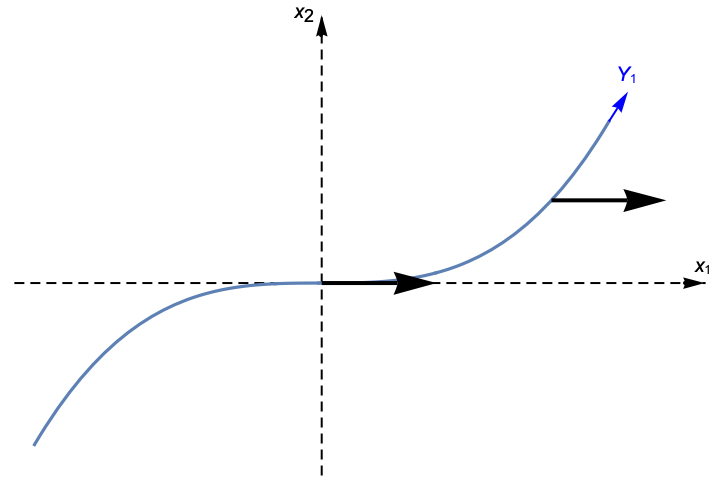
\includegraphics[width=7cm, height=5cm]{curvedaxis.png}
%    \caption{\textit{Στο επίπεδο σύστημα αναφοράς x %(διακεκομμένο) οι συνιστώσες του διανύσματος δεν μεταβάλλονται %καθώς αυτό μετακινείται, ωστόσο, στο καμπύλο σύστημα y %αλλάζουν.}}
%    \label{fig:curvedaxis}
%\end{figure}
%Η ανεπάρκεια της μερικής παραγώγου, έκδηλη από το δεύτερο όρο %της \eqref{pdertrans}, δείνει το κίνητρο για την κατασκευή της %συναλλοίωτης παραγώγου. Εκείνο που χρειαζόμαστε, είναι ένας %ακόμη όρος που να αντιπροσωπεύει τις ενδογενούς μεταβολές του %συστήματος συντεταγμένων. 
%Στο παράδειγμα του σχήματος \ref{fig:curvedaxis} ένα διάνυσμα %μετατοπίζεται παράλληλα σε έναν επίπεδο (διακεκομμένο) και έναν %καμπυλωμένο (συνεχής) χώρο με συντεταγμένες $x$ και $y$, %αντίστοιχα. Το μέτρο και η διεύθυνση του διανύσματος δεν %αλλάζει διεύθυνση, ούτε μέτρο άρα στο επίπεδο σύστημα οι %συνιστώσες του είναι σταθερές
%\begin{equation*}
%    \pd{V\superscr{\nu}}{x\superscr{\mu}} \,=\, 0
%\end{equation*}
%Λόγω της καμπυλότητας του y συστήματος όμως, οι μερικές %παραγώγοι στο εν λόγω σύστημα δεν είναι σταθερές
%\begin{equation*}
%    \pd{V'^{\nu}}{\y\superscr{\mu}} \,\neq\, 0
%\end{equation*}
\\

Επειδή η μερική παράγωγος μπορεί να είναι μηδενική σε κάποιο σύστημα αναφοράς συντεταγμένων και μη μηδενική σε κάποιο άλλο, δεν μπορεί να είναι τανυστής. Μπορούμε όμως να ορίσουμε τις συναλλοίωτες παραγώγους ανταλλοίωτων και συναλλοίωτων διανυσμάτων, οι οποίες μετασχηματίζονται ως τανυστές: 
%να εκφράσουμε τις μεταβολές συναλλοίωτου τανυστή πρώτης τάξης, %ως εξής 
\begin{equation}\label{covdevcov}
    \nabla\indices{_\mu}V\subscr{\nu} = \pd{V\subscr{\nu}}{x\superscr{\mu}} - \Gamma\indices{^\alpha_\mu_\nu} V\subscr{\alpha}
\end{equation}
ενώ για ανταλλοίωτο τανυστή πρώτης τάξης
\begin{equation}\label{covdevcont}
    \nabla\indices{_\mu}V\superscr{\nu} = \pd{V\superscr{\nu}}{x\superscr{\mu}} + \Gamma\indices{^\nu_\mu_\alpha} V\superscr{\alpha}
\end{equation}
%όπου τα πρόσιμα καθορίζονται βάση σύμβασης. Αναφερόμαστε στις %δύο πιο πάνω εκφράσεις ως η συναλλοίωτη παράγωγος, συναλλοίωτου %και ανταλλοίωτου τανυστή, αντίστοιχα. Ο δεύτερος όρος περιέχει 
Τα στοιχεία $\Gamma\indices{^\rho_\sigma_\lambda}$ ορίζονται με τέτοιο τρόπο, ώστε οι συναλλοίωτες παράγωγοι \eqref{covdevcov} και \eqref{covdevcont} να μετασχηματίζονται ως τανυστές. Για παράδειγμα,
\begin{equation*}
    \nabla\indices{_\mu}V\superscr{\nu} \rightarrow \L[i]{\alpha}{\mu}\L{\nu}{\beta}\nabla\indices{_\alpha}V\superscr{\beta}
\end{equation*}
Τα στοιχεία $\Gamma\indices{^\rho_\sigma_\lambda}$ είναι γνωστά και ως σύμβολα Christoffel. Δεν αποτελούν τις συνιστώσες κάποιου τανυστή, αφού δεν μετασχηματίζονται ανάλογα. Η γενίκευση των \eqref{covdevcov} και \eqref{covdevcont} για τανυστές μεγαλύτερης τάξης επιτυγχένεται άμεσα. Για παάδειγμα, στην περίπτωση τανυστή τέταρτης τάξης, παίρνουμε
\begin{equation*}
    \nabla\subscr{\lambda}T\indices{^\mu_\rho^\nu_\sigma} \,=\, \pd{\,}{x\superscr{\lambda}} T\indices{^\mu_\rho^\nu_\sigma}+ \Gamma\indices{^\mu_\lambda_\alpha}T\indices{^\alpha_\rho^\nu_\sigma} - \Gamma\indices{^\alpha_\lambda_\rho}T\indices{^\mu_\alpha^\nu_\sigma} + \Gamma\indices{^\nu_\lambda_\alpha}T\indices{^\mu_\rho^\alpha_\sigma} - \Gamma\indices{^\alpha_\lambda_\sigma}T\indices{^\mu_\rho^\nu_\alpha}
\end{equation*}